%%%%%%%%%%%%%%%%%%%%%%%%%%%%%%%%%%%%%%%%%
% a0poster Portrait Poster
% LaTeX Template
% Version 1.0 (22/06/13)
%
% The a0poster class was created by:
% Gerlinde Kettl and Matthias Weiser (tex@kettl.de)
% 
% This template has been downloaded from:
% http://www.LaTeXTemplates.com
%
% License:
% CC BY-NC-SA 3.0 (http://creativecommons.org/licenses/by-nc-sa/3.0/)
%
%%%%%%%%%%%%%%%%%%%%%%%%%%%%%%%%%%%%%%%%%

%----------------------------------------------------------------------------------------
%	PACKAGES AND OTHER DOCUMENT CONFIGURATIONS
%----------------------------------------------------------------------------------------

\documentclass[a0,portrait]{a0poster}

\usepackage{multicol} % This is so we can have multiple columns of text side-by-side
\columnsep=100pt % This is the amount of white space between the columns in the poster
\columnseprule=3pt % This is the thickness of the black line between the columns in the poster

\usepackage[svgnames]{xcolor} % Specify colors by their 'svgnames', for a full list of all colors available see here: http://www.latextemplates.com/svgnames-colors

\usepackage{times} % Use the times font
%\usepackage{palatino} % Uncomment to use the Palatino font

\usepackage{graphicx} % Required for including images
\graphicspath{{figures/}} % Location of the graphics files
\usepackage{booktabs} % Top and bottom rules for table
\usepackage[font=small,labelfont=bf]{caption} % Required for specifying captions to tables and figures
\usepackage{amsfonts, amsmath, amsthm, amssymb} % For math fonts, symbols and environments
\usepackage{wrapfig} % Allows wrapping text around tables and figures
\usepackage{xcolor}
\usepackage{tcolorbox}



\begin{document}

%----------------------------------------------------------------------------------------
%	POSTER HEADER 
%----------------------------------------------------------------------------------------

% The header is divided into two boxes:
% The first is 75% wide and houses the title, subtitle, names, university/organization and contact information
% The second is 25% wide and houses a logo for your university/organization or a photo of you
% The widths of these boxes can be easily edited to accommodate your content as you see fit

\begin{minipage}[b]{0.85\linewidth}
\veryHuge \color{NavyBlue} \textbf{Stellar oscillations induced by a planetary companion} \color{Black}\\ % Title
\Huge\textit{Going off on a tangent}\\[1cm] % Subtitle
\huge \textbf{Andrew Bunting\textsuperscript{1}, John Papaloizou\textsuperscript{2} \& Caroline Terquem\textsuperscript{1}}\\[0.5cm] % Author(s)
\Large \textsuperscript{1}Physics Department, University of Oxford; \textsuperscript{2}DAMPT, University of Cambridge\\[0.4cm] % University/organization
\Large andrew.bunting@physics.ox.ac.uk\\
\end{minipage}
%
\begin{minipage}[b]{0.15\linewidth}

\includegraphics[width=0.8\linewidth]{ox_logo.png}\\
\vspace{2.5cm}
\end{minipage}

\vspace{0.0cm} % A bit of extra whitespace between the header and poster content

%----------------------------------------------------------------------------------------

\begin{multicols}{2} % This is how many columns your poster will be broken into, a portrait poster is generally split into 2 columns

%----------------------------------------------------------------------------------------
%	ABSTRACT
%----------------------------------------------------------------------------------------

\color{black} % Navy color for the abstract


\begin{tcolorbox}[colframe=black,colback=blue!10!white]

\vspace{0.5cm}

\section*{Abstract}
\large
The gravitational potential from a planet orbiting a star causes a regular perturbation which results in oscillations in the star. In solving the non-adiabatic oscillation equations we found that the horizontal displacement at the surface is $\sim 10^{2} - 10^{3}$ times larger than the adiabatic solution. This result agrees well with analytical expressions which are valid at the surface boundary. These tidally induced oscillations cause changes in the observed brightness and radial velocity of the star. Modelling these oscillations could be used to characterise exoplanetary orbits, including determining planetary masses, and could potentially be used for planetary detection.
\normalsize

\vspace{0.5cm}

\end{tcolorbox}

%----------------------------------------------------------------------------------------
%	INTRODUCTION
%----------------------------------------------------------------------------------------

\color{Black} % SaddleBrown color for the introduction

\begin{tcolorbox}[colframe=black,colback=blue!10!white]

\vspace{0.5cm}

\section*{Introduction}

Both the radial velocity (RV) and transit methods for detecting exoplanets have been successful, but both are limited -- characterising the planet's mass is a particular difficulty due to degeneracy with the inclination or the density, respectively. Understanding other star-planet interactions, such as tidal oscillations, could break these degeneracies.

Given their mass, size and proximity to their host star, hot Jupiters have a stronger interaction with their host star than other planets. The first-order effect of their presence is what is used to detect them in both the RV and transit methods -- the motion of the star around the common centre of mass, and the light blocked by their presence respectively. The tidal potential due to the planet is a second-order effect which deforms the star (causing material to be displaced both radially and horizontally) and changes the amplitude and wavelength of the star's light. This changes the star's observed brightness and radial velocity.

Whilst modelling this interaction for the non-adiabatic case has been undertaken before \textsuperscript{\cite{Pfahl2008}}, a detailed analysis of the horizontal displacement has been lacking, or has otherwise been done assuming that the change due to non-adiabaticity is small \textsuperscript{\cite{Terquem1998}}.

This work particularly focusses upon the behaviour at the very surface, where non-adiabatic effects are prominent. Comparison between the modelled behaviour and analytical results under the conditions present at the very surface show good agreement.

\vspace{0.5cm}

\end{tcolorbox}


%----------------------------------------------------------------------------------------
%	METHOD
%----------------------------------------------------------------------------------------

\color{DarkSlateGray} % DarkSlateGray color for the rest of the content

\begin{tcolorbox}[colframe=black,colback=blue!10!white]

\vspace{0.5cm}

\section*{Method}

%------------------------------------------------

\subsection*{Numerical method}

To model the oscillations, the linear non-adiabatic stellar oscillation equations were solved in the case that the star is perturbed by a regular tidal potential, due to the planet. The variables directly solved for are: $\xi_{r}$, the radial displacement; $F_{r}'$, the perturbation to the radial radiative flux; $p'$, the perturbation to the pressure; and $T'$, the perturbation to the temperature.

The equations solved are:

\small
\begin{equation} \label{eq:cont_osc}
\frac{1}{r^{2}} \frac{\partial}{\partial r} ( r^{2} \rho_{0} \xi_{r} )  
+ \left( \frac{\rho_{0}}{\chi_{\rho} p_{0}} - \frac{l (l+1)}{m^{2} \omega^{2} r^{2}} \right) p'
- \frac{\rho_{0}}{T_{0}} \frac{\chi_{T}}{\chi_{\rho}} T'
=
\frac{l (l+1)}{m^{2} \omega^{2} r^{2}} \rho_{0} \Phi_{P}
\end{equation}
\\
\begin{equation} \label{eq:ent_osc}
\left( i \rho_{0} m \omega c_{p}  + \frac{l (l+1)}{r^{2}} K_{0} \right) T'
- \left( i m \omega c_{p} \nabla_{ad} \rho_{0} T_{0}  \right) \frac{p'}{p_{0}}
+ i m \omega \rho_{0} T_{0} \frac{\partial s_{0}}{\partial r} \xi_{r}
+ \frac{1}{r^{2}} \frac{\partial}{\partial r} ( r^{2} F_{r}')
=
0
\end{equation}
\\
\begin{multline} \label{eq:flux_osc}
 \frac{F_{r}'}{K_{0}}
- \left( \frac{\partial}{\partial r} - \frac{1}{T_{0}} \frac{\partial T_{0}}{\partial r} \left[ -3 + \frac{1}{\kappa_{0}} \left( \frac{\partial \kappa}{\partial \ln T} \right)_{\rho} - \frac{\chi_{T}}{\chi_{\rho}} \left( 1 + \frac{1}{\kappa_{0}} \left( \frac{\partial \kappa}{\partial \ln \rho} \right)_{T} \right) \right] \right) T' 
- \frac{\partial T_{0}}{\partial r} \frac{1}{p_{0} \chi_{\rho}} \left( 1 + \frac{1}{\kappa_{0}} \left( \frac{\partial \kappa}{\partial \ln \rho} \right)_{T} \right) p'
=
0
\end{multline}
\\
\begin{equation} \label{eq:mom_osc}
- m^{2} \omega^{2} \rho_{0} \xi_{r} 
+ \left( \frac{\partial}{\partial r} + \frac{\rho_{0}}{\chi_{\rho} p_{0}} \frac{\partial \Phi_{0}}{\partial r} \right) p'
-  \frac{\partial \Phi_{0}}{\partial r} \frac{\rho_{0}}{T_{0}} \frac{\chi_{T}}{\chi_{\rho}} T'
=
- \rho_{0} \frac{\partial \Phi_{P}}{\partial r}
\end{equation}
\\
\normalsize
which correspond to the continuity equation, entropy equation, radiative diffusion equation, and the momentum equation respectively.


The boundary conditions are split, two apply at the centre, and two at the surface. At the centre $\xi_{r} = 0$ and $F_{r}' = 0$ which ensure continuity. At the surface $\Delta P = 0$, ensuring that the pressure at the perturbed surface is unchanged, and $\left( 4 \frac{\Delta T}{T_{0}} - \frac{\Delta F_{r}}{F_{r_{0}}} \right) = 0$, ensuring that the star remains a blackbody emitter.

The Henyey method \textsuperscript{\cite{Henyey1964}} was used to solve these equations, using a solar-type model produced using MESA \textsuperscript{\cite{Paxton2011}} as the equilibrium background star which we perturbed.

%------------------------------------------------

\subsection*{Analytical solution}

For the region at the surface, analytical expressions for the relationships between variables can be found.  Our analysis has produced an expression for the ratio between the horizontal and radial displacements which is fully non-adiabatic.

These expressions have been compared to the output produced by the numerical model, and have been found to be in agreement.

\vspace{0.5cm}

\end{tcolorbox}



 %----------------------------------------------------------------------------------------
%	REFERENCES
%----------------------------------------------------------------------------------------

\begin{tcolorbox}[colframe=black,colback=blue!10!white]
\small
%\nocite{*} % Print all references regardless of whether they were cited in the poster or not
\bibliographystyle{plain} % Plain referencing style
\bibliography{library} % Use the example bibliography file sample.bib
\normalsize

\end{tcolorbox}



%----------------------------------------------------------------------------------------
%	RESULTS 
%----------------------------------------------------------------------------------------

\begin{tcolorbox}[colframe=black,colback=blue!10!white]

\vspace{0.5cm}

\section*{Results}

The results shown here are for a solar-type star, orbited by a Jupiter mass planet with a period of $4.23$ days. The behaviour in the last $0.1\%$ of the stellar radius differs greatly between the adiabatic and non-adiabatic cases. The inclusion of non-adiabaticity leads to the radial displacement, $\xi_{r}$, being suppressed relative to the equilibrium value (by a factor of $\sim 10$), and the horizontal displacement, $\xi_{h}$, is amplified (by a factor of $\sim 10^{2} - 10^{3}$).

A rough estimate for the ratio $\frac{\xi_{h}}{\xi_{r}} \sim \frac{r}{H_{p}}$, where $H_{p}$ is the pressure scale height gives a surface value of $\sim 5000$, which is the right order of magnitude, as seen in figure \ref{fig:displacements}. Using the more involved expression derived in our analysis, we get the more precise value of $3200 \pm 300$, compared to the model's value of $3000 \pm 50$, where the errors are due to numerical scatter in the output.

\begin{center}\vspace{1cm}
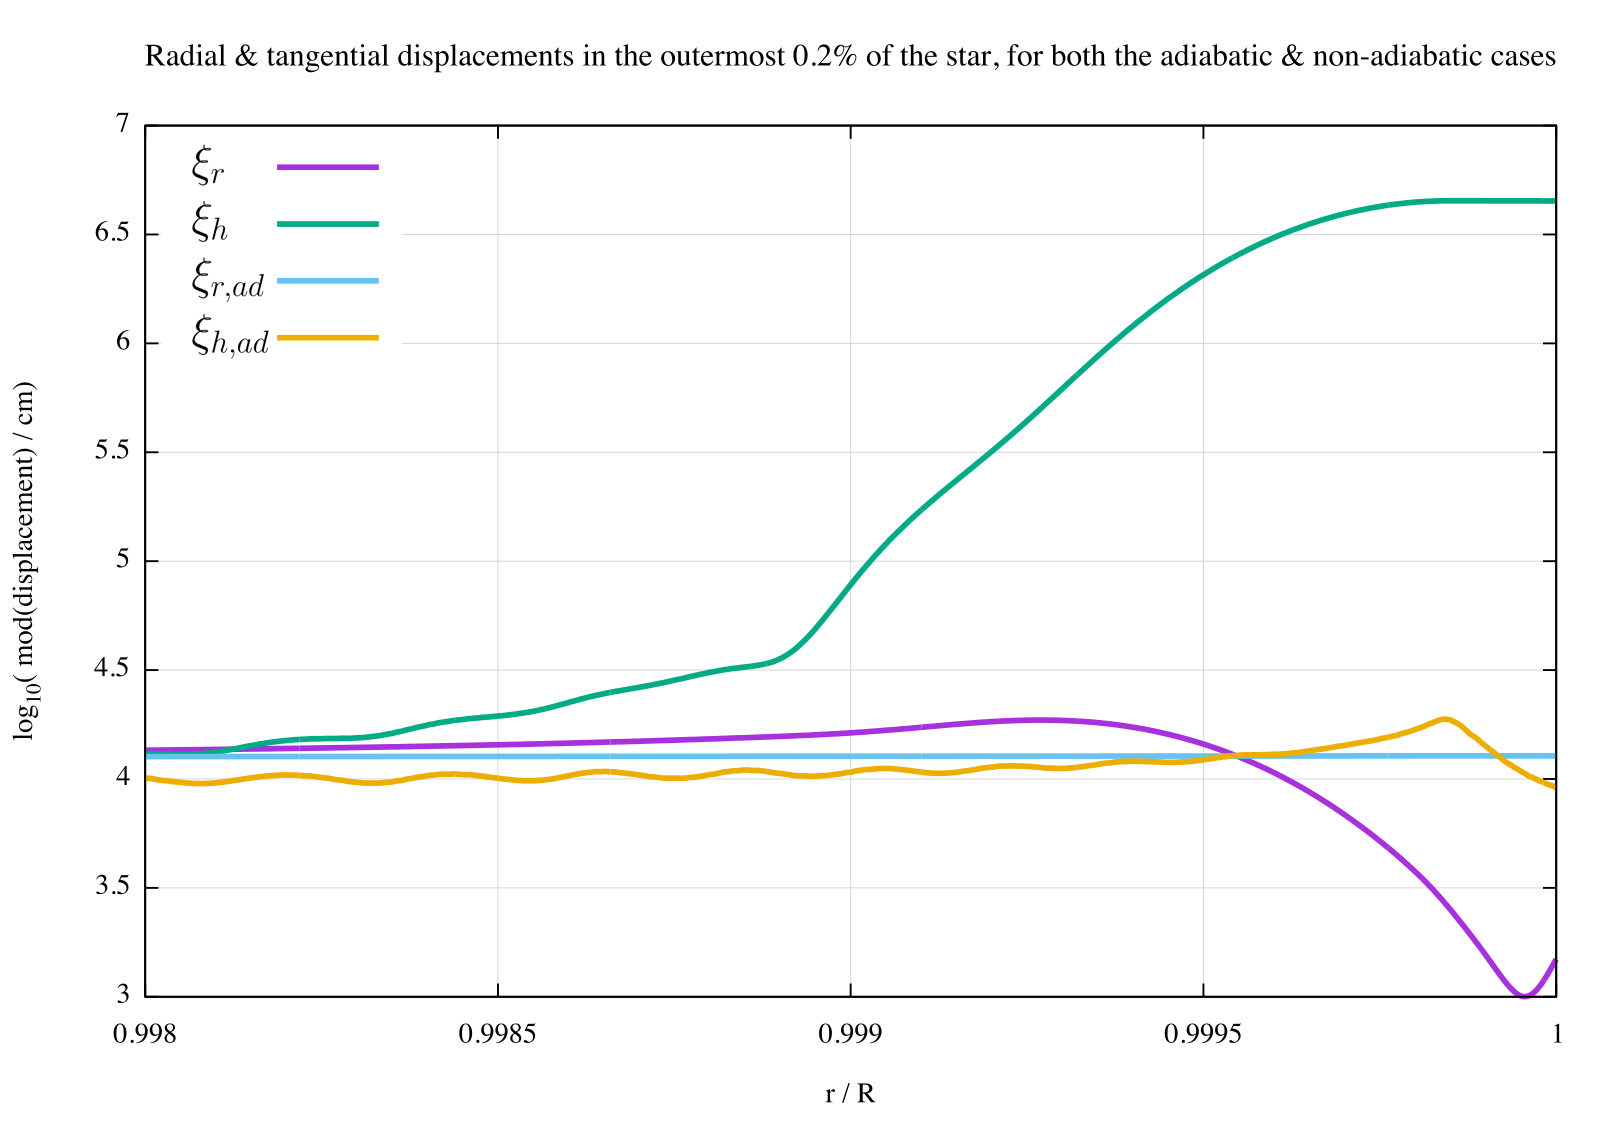
\includegraphics[width=0.98\linewidth]{poster_mod_displacements_key}
\captionof{figure}{\color{Black} A close-up of the surface of a solar-type star, showing the logarithms of the moduli of radial and horizontal displacements ($\xi_{r}$ and $\xi_{h}$, respectively) for both the non-adiabatic and the adiabatic case (denoted by the subscript ad). In the adiabatic case $\xi_{r,ad}$ and $\xi_{h,ad}$ are approximately similar at the surface. Taking non-adiabatic effects into account suppresses $\xi_{r}$, and greatly amplifies $\xi_{h}$ by a factor of $\sim 10^{2} - 10^{3}$.}
\label{fig:displacements}
\end{center}\vspace{1cm}

The significant departure from the adiabatic case is also seen in the phase of the surface behaviour, relative to the orbital motion. Both the radial and horizontal displacements lead the orbit, by $44^{\circ}$ and $86^{\circ}$ respectively. Because of this, any signal due to the tidal oscillations could be expected to be significantly phase-shifted relative to the orbital motion. Due to their differing dependences upon $\xi_{r}$ and $\xi_{h}$, the photometric and spectroscopic signals could be expected to have different phases as well. Such information could be useful in determining the mass of the planet causing the oscillations.

%Both $\xi_{r}$ and $\xi_{h}$ become negative in the surface region, leading to a phase shift of $90^{\circ}$ between the planetary motion and the surface response of the star. On top of this, the imaginary part of $\xi_{r}$ is of similar magnitude to the real part, leading to an additional phase shift of $48^{\circ}$. The horizontal displacement is dominated by its real part, leading to an additional phase shift of only $5^{\circ}$. In this case, this leads to the radial displacement leading the orbital motion by $42^{\circ}$, and the horizontal displacement leading by $85^{\circ}$. As such, any signal, whether photometric or spectroscopic, could be expected to be significantly phase-shifted with respect to the orbital motion.

\begin{center}\vspace{1.0cm}
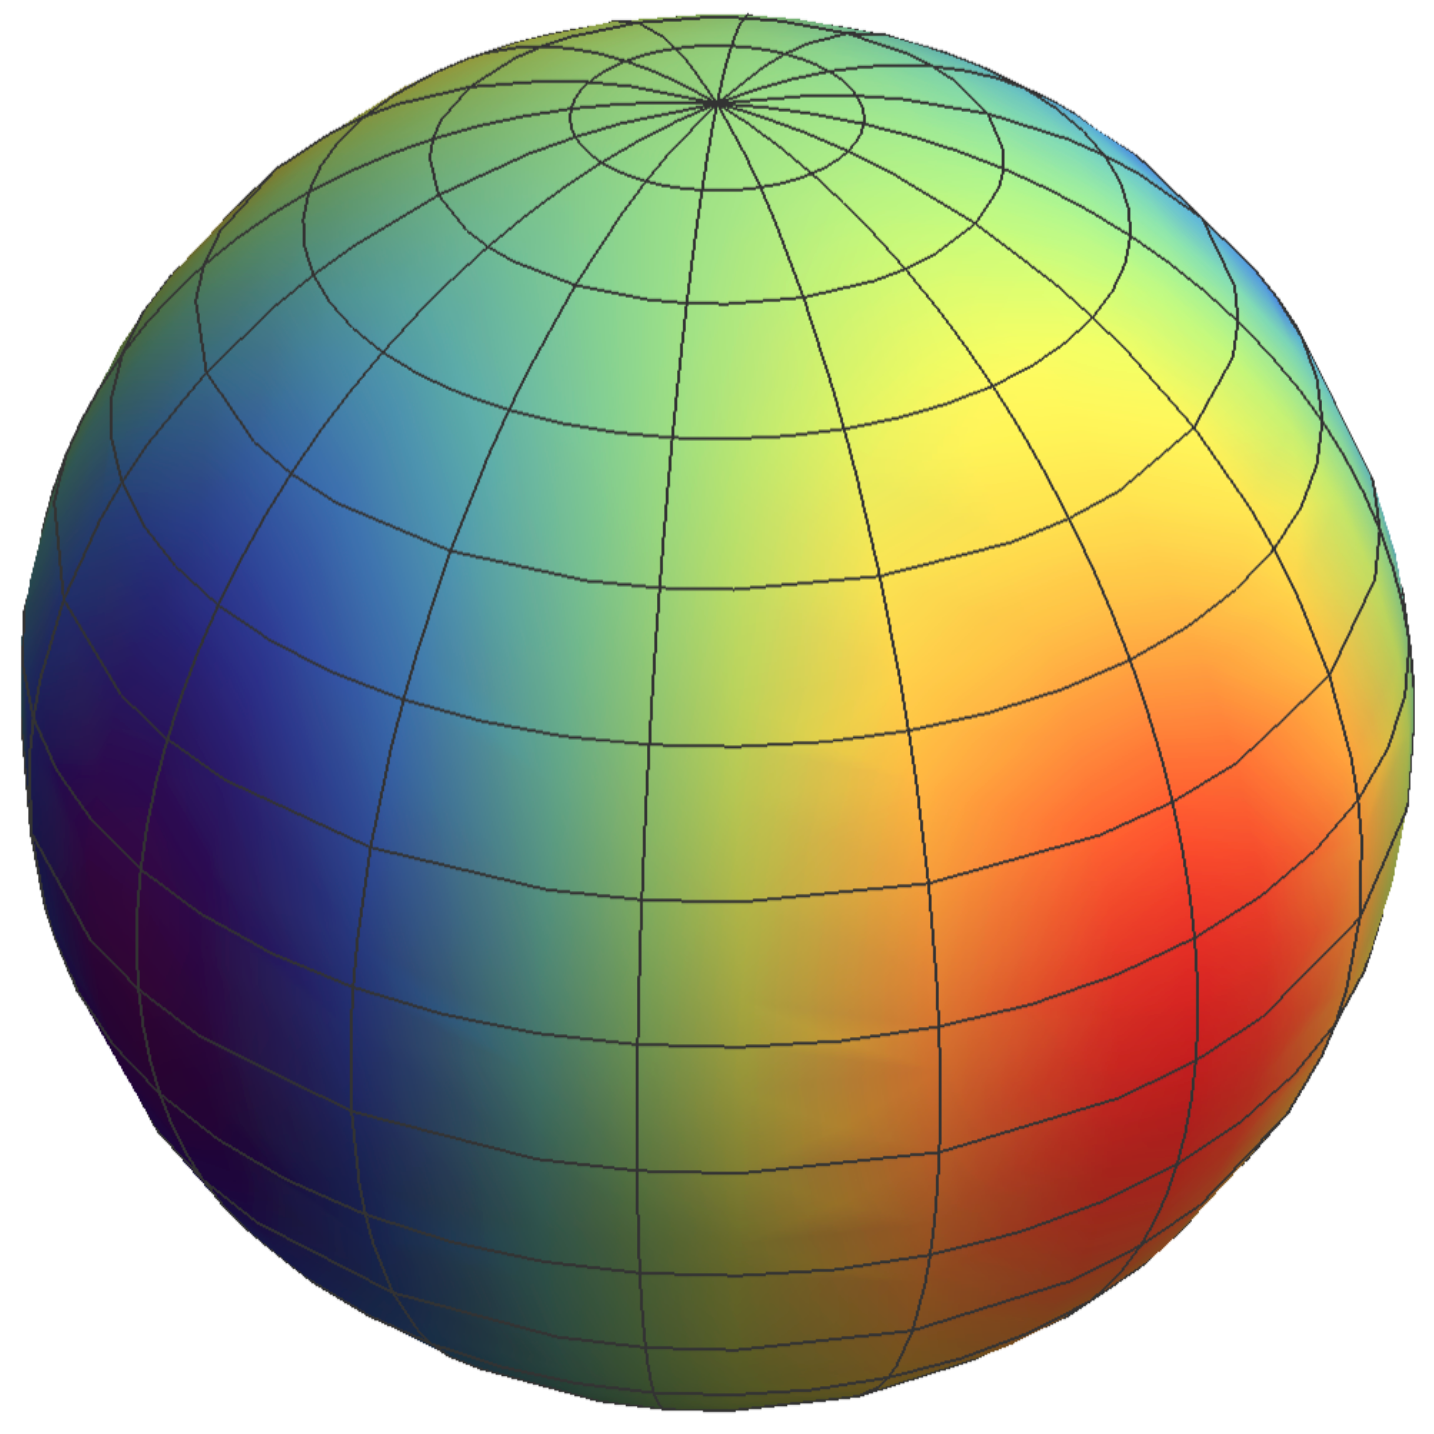
\includegraphics[width=0.45\linewidth]{radial_map_complex_crop_transp}
~
~
~
~
~
~
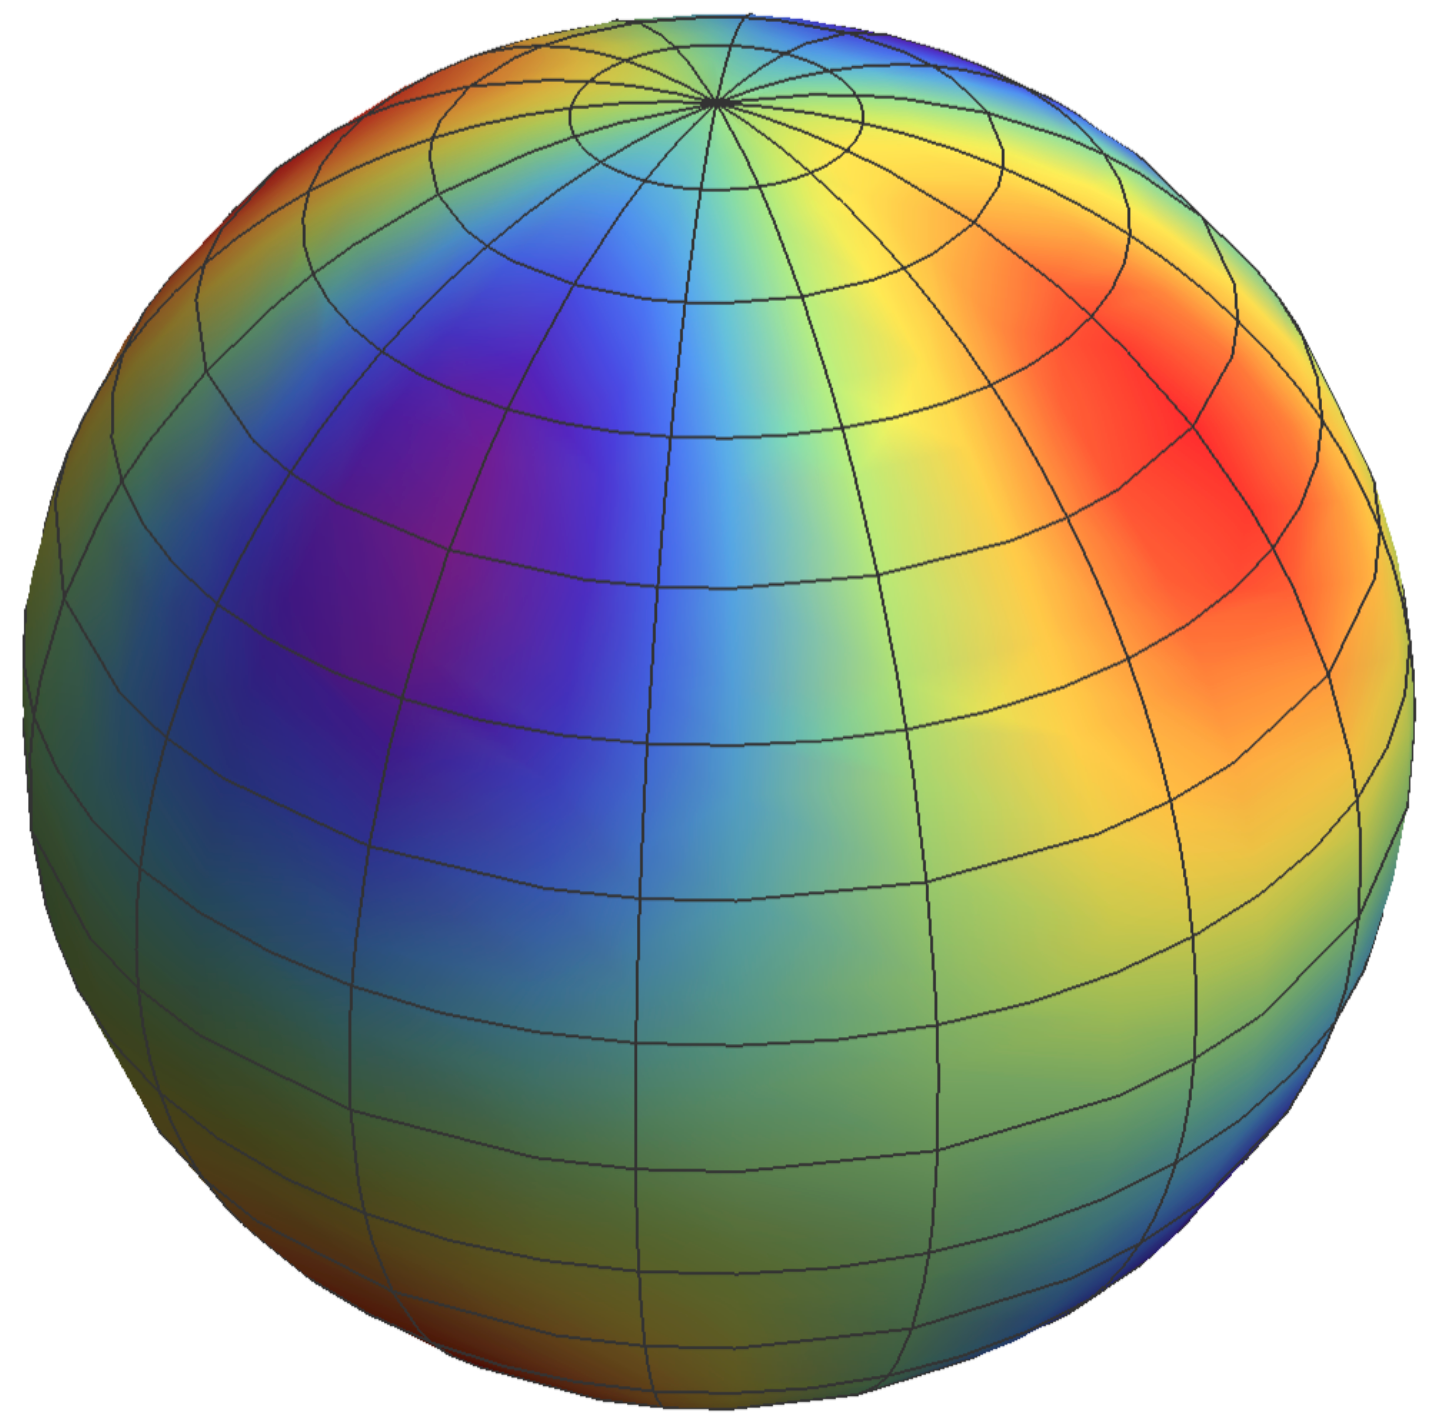
\includegraphics[width=0.45\linewidth]{tangential_map_complex_crop_transp}
\captionof{figure}{\color{Black} A heat map showing the distribution on the surface of the star of radial displacement ($\xi_{r}$, left, corresponding to $\sin^{2}(\theta) \cos(2 \phi + \phi_{r})$, where $\phi_{r}$ is the argument of $\xi_{r}$ at the surface) and horizontal displacement ($\xi_{h}$, right, corresponding to $\sin(\theta) \cos(\theta) \cos(2 \phi + \phi_{h})$ where $\phi_{h}$ is the argument of $\xi_{h}$ at the surface). Blue and red correspond to the large amplitudes of opposite phase. The radial displacement leads the orbital motion by $44^{\circ}$, whereas the horizontal displacement leads by $86^{\circ}$. The ratio of amplitudes $\frac{\xi_{h}}{\xi_{r}} \sim 10^{3}$.}
\label{fig:maps}
\end{center}\vspace{1.0cm}


Due to the spatial distribution of the horizontal displacement (shown in figure \ref{fig:maps}), it averages out when integrated over the visible disk. Therefore it does not contribute to a change in overall brightness, and the suppression of $\xi_{r}$ implies that such variation may be difficult to find. The horizontal displacement would contribute to the radial velocity signal, however, and suggests that this signal could be larger than previously anticipated.

\vspace{0.5cm}

\end{tcolorbox}

%----------------------------------------------------------------------------------------
%	CONCLUSIONS
%----------------------------------------------------------------------------------------

\color{Black}

\begin{tcolorbox}[colframe=black,colback=blue!10!white]

\vspace{0.5cm}

\section*{Conclusions}

\large

\begin{itemize}
\item Non-adiabatic effects have a strong impact upon the behaviour of oscillations at the surface
\item Horizontal displacement is increased by a factor of $\sim 10^{2} - 10^{3}$ compared to the equilibrium tide
\item The numerical results agree well with analytical expressions at the surface
\item These oscillations would be visible as changes in brightness and radial velocity
\item This could be used to characterise or detect planetary systems (work in progress)
\end{itemize}
\vspace{0.5cm}

\normalsize

\end{tcolorbox}

\color{Black} % Set the color back to DarkSlateGray for the rest of the content

%----------------------------------------------------------------------------------------
%	FORTHCOMING RESEARCH
%----------------------------------------------------------------------------------------



%----------------------------------------------------------------------------------------
%	ACKNOWLEDGEMENTS
%----------------------------------------------------------------------------------------



%----------------------------------------------------------------------------------------

\end{multicols}
\end{document}